%!TEX program = xelatex
\documentclass[11pt, a4paper]{article}

% AA LINGUA E GESTIONE FONT (Specifica per XeLaTeX)
\usepackage{fontspec}
\setmainfont{Latin Modern Roman}
\usepackage[italian]{babel}

% AA LAYOUT DI PAGINA E TIPOGRAFIA (Ottimizzato per Rilegatura)
\usepackage[left=2.4cm, right=1.6cm, top=2cm, bottom=2cm]{geometry}

% AA Spaziatura tra paragrafi controllata (compatta ed evita salti enormi)
\usepackage[skip=3pt plus 1pt minus 1pt]{parskip}
\setlength{\parindent}{0pt}

% AA Microtype per XeLaTeX
\usepackage[protrusion=true]{microtype}
\raggedbottom

% AA GESTIONE DEI COLORI
\usepackage{xcolor}

% BB COLORI E MACRO PER I SIGMA
\definecolor{sigRed}{RGB}{215, 0, 0}
\definecolor{sigBlue}{RGB}{0, 70, 220}
\definecolor{sigGreen}{RGB}{0, 145, 45}

\newcommand{\sigA}{\textcolor{sigRed}{\boldsymbol{\sigma_A}}}
\newcommand{\sigB}{\textcolor{sigBlue}{\boldsymbol{\sigma_B}}}
\newcommand{\sigC}{\textcolor{sigGreen}{\boldsymbol{\sigma_C}}}

% AA MATEMATICA E SIMBOLI
\usepackage{amsmath}
\usepackage{mathtools}
\usepackage{silence}
\usepackage[warnings-off={mathtools-overbracket,mathtools-colon}]{unicode-math}
\setmathfont{Latin Modern Math}

% BB OTTIMIZZAZIONE MATRICI LUNGHE PER LA STAMPA
\setlength{\arraycolsep}{10pt}

% AA Spaziature verticali attorno alle formule matematiche
\setlength{\abovedisplayskip}{3pt plus 1pt minus 1pt}
\setlength{\belowdisplayskip}{3pt plus 1pt minus 1pt}
\setlength{\abovedisplayshortskip}{0pt plus 1pt}
\setlength{\belowdisplayshortskip}{2pt plus 1pt minus 1pt}

% AA GRAFICA ED IMMAGINI
\usepackage{graphicx}
\graphicspath{{./E3_2_Images/}}

% AA PERSONALIZZAZIONE TITOLI
\usepackage{titlesec}
\titleformat{\section}{\normalfont\Large\bfseries\color{blue!80!black}}{\thesection}{1em}{}
\titleformat{name=\section,numberless}{\normalfont\Large\bfseries\color{blue!80!black}}{}{0pt}{}

\titleformat{\subsection}{\normalfont\large\bfseries}{\thesubsection}{1em}{}
\titleformat{name=\subsection,numberless}{\normalfont\large\bfseries}{}{0pt}{}

\titleformat{\subsubsection}{\normalfont\normalsize\bfseries}{\thesubsubsection}{1em}{}
\titleformat{name=\subsubsection,numberless}{\normalfont\normalsize\bfseries}{}{0pt}{}

\titlespacing*{\section}{0pt}{1.2ex plus 0.4ex minus 0.2ex}{0.6ex plus 0.2ex}
\titlespacing*{\subsection}{0pt}{1ex plus 0.3ex minus 0.2ex}{0.5ex plus 0.2ex}
\titlespacing*{\subsubsection}{0pt}{0.8ex plus 0.2ex minus 0.1ex}{0.4ex plus 0.1ex}

\titleformat{\paragraph}[block]{\normalfont\normalsize\bfseries\color{black!80!black}\raggedright}{}{0pt}{}
\titlespacing*{\paragraph}{0pt}{1.2ex plus 0.3ex minus 0.2ex}{0.4ex}

% AA INTEGRAZIONE CODICE MATLAB
\usepackage{matlab}

% BB Riconfigurazione Automatica Titoli Esportati da MATLAB
\renewcommand{\matlabheading}[1]{\section*{#1}}
\renewcommand{\matlabheadingtwo}[1]{\subsection*{#1}}
\renewcommand{\matlabheadingthree}[1]{\subsubsection*{#1}}

% BB Formule E Matrici Simboliche
\renewenvironment{matlabsymbolicoutput}{%
  \par\vspace{2pt}%
  \begingroup
  \centering
}{%
  \par\vspace{2pt}%
  \endgroup
}

% BB Output Testuale Console
\renewenvironment{matlaboutput}{%
  \par\vspace{1pt}%
  \Verbatim[xleftmargin=10pt, formatcom=\color{black!75}, fontsize=\footnotesize]%
}{%
  \endVerbatim
  \vspace{1pt}%
}

% BB Box Codice (Stile Moderno con Barra Laterale Colorata)
\lstset{
  backgroundcolor={},
  aboveskip=0pt,
  belowskip=0pt,
  basicstyle=\ttfamily\footnotesize,
  xleftmargin=0pt
}

\mdfdefinestyle{matlabcode}{%
  topline=false,
  bottomline=false,
  rightline=false,
  leftline=true,
  linewidth=2.5pt,
  linecolor=blue!75!black,
  backgroundcolor=black!3,
  innertopmargin=4pt,
  innerbottommargin=4pt,
  innerleftmargin=9pt,
  innerrightmargin=6pt,
  skipabove=3pt,
  skipbelow=3pt
}

\allowdisplaybreaks

% AA LINK, METADATI ED ELENCHI
\usepackage{hyperref}
\hypersetup{
    colorlinks=true,
    linkcolor=blue!80!black,
    urlcolor=blue!80!black,
    citecolor=blue!80!black,
    pdftitle={Cinematica Diretta Manipolatore SCARA},
    pdfauthor={Francesco Lo Verde},
}
\usepackage{bookmark}

% BB Spaziatura Elenchi (Arieggiata per la Stampa)
\usepackage{enumitem}
\setlist{itemsep=3.5pt plus 1pt minus 1pt, topsep=4pt plus 1pt minus 1pt, partopsep=0pt, parsep=1pt}


\author{Francesco Lo Verde}
\begin{document}


\matlabtitle{Calcolo Cinematica Diretta Con Parametri Di Denavit-Hartenberg}

\begin{par}
\begin{flushleft}
L'obiettivo della cinematica diretta è determinare la posizione e l'orientamento dell'organo terminale (end-effector) a partire dai valori delle variabili di giunto. Si utilizza la convenzione di Denavit-Hartenberg (DH) per modellare la geometria del robot. La convenzione di Denavit-Hartenberg è un metodo standard per assegnare sistemi di riferimento ai bracci di un robot. Per ogni braccio, si definiscono quattro parametri che descrivono la trasformazione geometrica rispetto al braccio precedente.
\end{flushleft}
\end{par}

\begin{par}
\begin{flushleft}
Si inizia definendo le variabili simboliche necessarie per i parametri DH. Questo permette di eseguire i calcoli in forma generale, senza dover specificare subito valori numerici. Successivamente, si assemblano questi parametri in una tabella dove ogni riga corrisponde a un giunto del robot e le colonne rappresentano i parametri $\left(\begin{array}{c}
\theta ,d,\alpha ,a
\end{array}\right)$.
\end{flushleft}
\end{par}

\begin{matlabcode}
clc;
clear;
close all;

% Definizione Variabili Simboliche
syms q1 q2 q3 q4 d1 d2 d3 d4 a1 a2 a3 a4 real;

% Tabella Parametri Denavit-Hartenberg (DH)
% Le colonne sono: [theta, d, a, alpha]
DH_table = [q1, d1, a1, 0;
            q2, 0,  a2, 0;
            0,  q3, 0,  0;
            q4, d4, 0,  pi];

% Numero Giunti Manipolatore
n = size(DH_table, 1);
\end{matlabcode}

\begin{par}
\begin{flushleft}
A partire dalla tabella DH, si può calcolare la matrice di trasformazione omogenea $A_i$ per ciascun giunto $i$. Questa matrice, di dimensioni $4\times 4$ e rappresenta la trasformazione (rotazione e traslazione) dal sistema di riferimento del giunto $i$ a quello del giunto $i-1$. Si utilizza la funzione \texttt{Compute\_DH\_Transformations} per generare le matrici simboliche per ogni riga della tabella DH.
\end{flushleft}
\end{par}

\begin{matlabcode}
[T_matrices, R_matrices] = Compute_DH_Transformations(DH_table);

for i = 1:n
    fprintf('Matrice Di Trasformazione Omogenea ^(%d)T_(%d):\n', i-1, i);
    disp(T_matrices(:,:,i));
end
\end{matlabcode}
\begin{matlaboutput}
Matrice Di Trasformazione Omogenea ^(0)T_(1):
\end{matlaboutput}
\begin{matlabsymbolicoutput}
\hskip1em $\displaystyle \left(\begin{array}{cccc}
\cos \left(q_1 \right) & -\cos \left(a_1 \right)\,\sin \left(q_1 \right) & \sin \left(a_1 \right)\,\sin \left(q_1 \right) & 0\\
\sin \left(q_1 \right) & \cos \left(a_1 \right)\,\cos \left(q_1 \right) & -\sin \left(a_1 \right)\,\cos \left(q_1 \right) & 0\\
0 & \sin \left(a_1 \right) & \cos \left(a_1 \right) & d_1 \\
0 & 0 & 0 & 1
\end{array}\right)$
\end{matlabsymbolicoutput}
\begin{matlaboutput}
Matrice Di Trasformazione Omogenea ^(1)T_(2):
\end{matlaboutput}
\begin{matlabsymbolicoutput}
\hskip1em $\displaystyle \left(\begin{array}{cccc}
\cos \left(q_2 \right) & -\cos \left(a_2 \right)\,\sin \left(q_2 \right) & \sin \left(a_2 \right)\,\sin \left(q_2 \right) & 0\\
\sin \left(q_2 \right) & \cos \left(a_2 \right)\,\cos \left(q_2 \right) & -\sin \left(a_2 \right)\,\cos \left(q_2 \right) & 0\\
0 & \sin \left(a_2 \right) & \cos \left(a_2 \right) & 0\\
0 & 0 & 0 & 1
\end{array}\right)$
\end{matlabsymbolicoutput}
\begin{matlaboutput}
Matrice Di Trasformazione Omogenea ^(2)T_(3):
\end{matlaboutput}
\begin{matlabsymbolicoutput}
\hskip1em $\displaystyle \left(\begin{array}{cccc}
1 & 0 & 0 & 0\\
0 & 1 & 0 & 0\\
0 & 0 & 1 & q_3 \\
0 & 0 & 0 & 1
\end{array}\right)$
\end{matlabsymbolicoutput}
\begin{matlaboutput}
Matrice Di Trasformazione Omogenea ^(3)T_(4):
\end{matlaboutput}
\begin{matlabsymbolicoutput}
\hskip1em $\displaystyle \left(\begin{array}{cccc}
\cos \left(q_4 \right) & -\sin \left(q_4 \right) & 0 & \pi \,\cos \left(q_4 \right)\\
\sin \left(q_4 \right) & \cos \left(q_4 \right) & 0 & \pi \,\sin \left(q_4 \right)\\
0 & 0 & 1 & d_4 \\
0 & 0 & 0 & 1
\end{array}\right)$
\end{matlabsymbolicoutput}
\begin{matlabcode}

T04 = T_matrices(:,:,1) * T_matrices(:,:,2) * T_matrices(:,:,3) * T_matrices(:,:,4);
T04 = simplify(T04);

fprintf('Matrice Di Trasformazione Omogenea Totale ^(0)T_(4):\n');
disp(T04);
\end{matlabcode}
\begin{matlaboutput}
Matrice Di Trasformazione Omogenea Totale ^(0)T_(4):
\end{matlaboutput}
\begin{matlabsymbolicoutput}
\resizebox{\linewidth}{!}{%
$
\begin{pmatrix}
    \cos \left(q_4 \right)\,\sigma_4 -s\left(q_4 \right)\,\sigma_2  & -s\left(q_4 \right)\,\sigma_4 -c\left(q_4 \right)\,\sigma_2  & \sigma_1  & d_4 \,\sigma_1 +q_3 \,\sigma_1 -\pi \,s\left(q_4 \right)\,\sigma_2 +\pi \,c\left(q_4 \right)\,\sigma_4 \\
    c\left(q_4 \right)\,\sigma_5 -s\left(q_4 \right)\,\sigma_3  & -s\left(q_4 \right)\,\sigma_5 -c\left(q_4 \right)\,\sigma_3  & \sigma_9 -\sigma_{10} -\sigma_8  & \pi \,c\left(q_4 \right)\,\sigma_5 -q_3 \,{\left(\sigma_{10} -\sigma_9 +\sigma_8 \right)}-\pi \,s\left(q_4 \right)\,\sigma_3 -d_4 \,{\left(\sigma_{10} -\sigma_9 +\sigma_8 \right)}\\
    s\left(q_4 \right)\,\sigma_7 +s\left(a_1 \right)\,c\left(q_4 \right)\,s\left(q_2 \right) & c\left(q_4 \right)\,\sigma_7 -s\left(a_1 \right)\,s\left(q_2 \right)\,s\left(q_4 \right) & \sigma_6  & d_1 +d_4 \,\sigma_6 +q_3 \,\sigma_6 +\pi \,s\left(q_4 \right)\,\sigma_7 +\pi \,s\left(a_1 \right)\,c\left(q_4 \right)\,s\left(q_2 \right)\\
    0 & 0 & 0 & 1
\end{pmatrix}
$%
}

\vspace{0.5em}
\noindent Dove:
\vspace{-0.5em}

\[
\begin{aligned}
    \sigma_1    &= c\left(a_2 \right)\,s\left(a_1 \right)\,s\left(q_1 \right)+s\left(a_2 \right)\,c\left(q_1 \right)\,s\left(q_2 \right)+c\left(a_1 \right)\,s\left(a_2 \right)\,c\left(q_2 \right)\,s\left(q_1 \right) \\
    \sigma_2    &= c\left(a_2 \right)\,c\left(q_1 \right)\,s\left(q_2 \right)-s\left(a_1 \right)\,s\left(a_2 \right)\,s\left(q_1 \right)+c\left(a_1 \right)\,c\left(a_2 \right)\,c\left(q_2 \right)\,s\left(q_1 \right) \\
    \sigma_3    &= s\left(a_1 \right)\,s\left(a_2 \right)\,c\left(q_1 \right)+c\left(a_2 \right)\,s\left(q_1 \right)\,s\left(q_2 \right)-c\left(a_1 \right)\,c\left(a_2 \right)\,c\left(q_1 \right)\,c\left(q_2 \right) \\
    \sigma_4    &= c\left(q_1 \right)\,c\left(q_2 \right)-c\left(a_1 \right)\,s\left(q_1 \right)\,s\left(q_2 \right) \\
    \sigma_5    &= c\left(q_2 \right)\,s\left(q_1 \right)+c\left(a_1 \right)\,c\left(q_1 \right)\,s\left(q_2 \right) \\
    \sigma_6    &= c\left(a_1 \right)\,c\left(a_2 \right)-s\left(a_1 \right)\,s\left(a_2 \right)\,c\left(q_2 \right) \\
    \sigma_7    &= c\left(a_1 \right)\,s\left(a_2 \right)+c\left(a_2 \right)\,s\left(a_1 \right)\,c\left(q_2 \right) \\
    \sigma_8    &= c\left(a_1 \right)\,s\left(a_2 \right)\,c\left(q_1 \right)\,c\left(q_2 \right) \\
    \sigma_9    &= s\left(a_2 \right)\,s\left(q_1 \right)\,s\left(q_2 \right) \\
    \sigma_{10} &= c\left(a_2 \right)\,s\left(a_1 \right)\,c\left(q_1 \right)
\end{aligned}
\]
\end{matlabsymbolicoutput}

\begin{par}
\begin{flushleft}
La matrice di trasformazione omogenea totale $^1 T_4$ contiene tutte le informazioni sulla posa dell'organo terminale. Da essa possiamo estrarre due elementi chiave:
\end{flushleft}
\end{par}

\begin{itemize}
   \item La \textbf{matrice di rotazione R}, che definisce l'orientamento dell'organo terminale rispetto alla base. Corrisponde alla sottomatrice 3x3 in alto a sinistra.
   \item Il \textbf{vettore di posizione p}, che indica la posizione dell'origine del sistema di riferimento dell'organo terminale. Corrisponde alle prime tre righe della quarta colonna.
\end{itemize}
\newpage
\begin{matlabcode}
% Estrazione Vettore Posizione
p04 = T04(1:3, 4);
p04 = simplify(p04);
fprintf('Vettore Posizione p04:\n');
disp(p04);
\end{matlabcode}
\begin{matlaboutput}
Vettore Posizione p04:
\end{matlaboutput}
\begin{matlabsymbolicoutput}
\[
\begin{pmatrix}
    \sigma_1 \\[4pt]
    \sigma_2 \\[4pt]
    \sigma_3
\end{pmatrix}
\]
Dove:
\[
\begin{aligned}
\sigma_1 &= d_4 \sigA + q_3 \sigA - \pi s\left(q_4\right)\left[c\left(a_2\right)c\left(q_1\right)s\left(q_2\right) - s\left(a_1\right)s\left(a_2\right)s\left(q_1\right) + c\left(a_1\right)c\left(a_2\right)c\left(q_2\right)s\left(q_1\right)\right] \\
        &\quad + \pi c\left(q_4\right)\left(c\left(q_1\right)c\left(q_2\right) - c\left(a_1\right)s\left(q_1\right)s\left(q_2\right)\right) \\[6pt]
\sigma_2 &= \pi c\left(q_4\right)\left[c\left(q_2\right)s\left(q_1\right) + c\left(a_1\right)c\left(q_1\right)s\left(q_2\right)\right] - q_3 \sigB \\
        &\quad - \pi s\left(q_4\right)\left(s\left(a_1\right)s\left(a_2\right)c\left(q_1\right) + c\left(a_2\right)s\left(q_1\right)s\left(q_2\right) - c\left(a_1\right)c\left(a_2\right)c\left(q_1\right)c\left(q_2\right)\right) - d_4 \sigB \\[6pt]
\sigma_3 &= d_1 + d_4 \sigC + q_3 \sigC + \pi s\left(q_4\right)\left[c\left(a_1\right)s\left(a_2\right) + c\left(a_2\right)s\left(a_1\right)c\left(q_2\right)\right] + \pi s\left(a_1\right)c\left(q_4\right)s\left(q_2\right) \\[6pt]
\sigA    &= c\left(a_2\right)s\left(a_1\right)s\left(q_1\right) + s\left(a_2\right)c\left(q_1\right)s\left(q_2\right) + c\left(a_1\right)s\left(a_2\right)c\left(q_2\right)s\left(q_1\right) \\[4pt]
\sigB    &= c\left(a_2\right)s\left(a_1\right)c\left(q_1\right) - s\left(a_2\right)s\left(q_1\right)s\left(q_2\right) + c\left(a_1\right)s\left(a_2\right)c\left(q_1\right)c\left(q_2\right) \\[4pt]
\sigC    &= c\left(a_1\right)c\left(a_2\right) - s\left(a_1\right)s\left(a_2\right)c\left(q_2\right)
\end{aligned}
\]
\end{matlabsymbolicoutput}

% Estrazione Matrice Rotazione
\begin{matlabcode}
R04 = T04(1:3, 1:3);
R04 = simplify(R04);
fprintf('Matrice Rotazione R04:\n');
disp(R04);
\end{matlabcode}
\begin{matlaboutput}
Matrice Rotazione R04:
\end{matlaboutput}

\begin{matlabsymbolicoutput}
\[
\begin{pmatrix}
    c \left(q_4 \right)\,\sigma_3 - s\left(q_4 \right)\,\sigma_1 & -s\left(q_4 \right)\,\sigma_3 - c \left(q_4 \right)\,\sigma_1 & \sigA \\[6pt]
    c \left(q_4 \right)\,\sigma_4 - s\left(q_4 \right)\,\sigma_2 & -s\left(q_4 \right)\,\sigma_4 - c \left(q_4 \right)\,\sigma_2 & -\sigB \\[6pt]
    s\left(q_4 \right)\,\sigma_5 + s\left(a_1 \right)c \left(q_4 \right)s\left(q_2 \right) & c \left(q_4 \right)\,\sigma_5 - s\left(a_1 \right)s\left(q_2 \right)s\left(q_4 \right) & \sigC
\end{pmatrix}
\]

\vspace{-0.2em}
\noindent Dove:
\vspace{-0.4em}

\[
\begin{aligned}
\sigma_1 &= c \left(a_2 \right)c \left(q_1 \right)s\left(q_2 \right) - s\left(a_1 \right)s\left(a_2 \right)s\left(q_1 \right) + c \left(a_1 \right)c \left(a_2 \right)c \left(q_2 \right)s\left(q_1 \right) \\[3pt]
\sigma_2 &= s\left(a_1 \right)s\left(a_2 \right)c \left(q_1 \right) + c \left(a_2 \right)s\left(q_1 \right)s\left(q_2 \right) - c \left(a_1 \right)c \left(a_2 \right)c \left(q_1 \right)c \left(q_2 \right) \\[3pt]
\sigma_3 &= c \left(q_1 \right)c \left(q_2 \right) - c \left(a_1 \right)s\left(q_1 \right)s\left(q_2 \right) \\[3pt]
\sigma_4 &= c \left(q_2 \right)s\left(q_1 \right) + c \left(a_1 \right)c \left(q_1 \right)s\left(q_2 \right) \\[3pt]
\sigma_5 &= c \left(a_1 \right)s\left(a_2 \right) + c \left(a_2 \right)s\left(a_1 \right)c \left(q_2 \right) \\[3pt]
\sigA    &= c \left(a_2 \right)s\left(a_1 \right)s\left(q_1 \right) + s\left(a_2 \right)c \left(q_1 \right)s\left(q_2 \right) + c \left(a_1 \right)s\left(a_2 \right)c \left(q_2 \right)s\left(q_1 \right) \\[3pt]
\sigB    &= c \left(a_2 \right)s\left(a_1 \right)c \left(q_1 \right) - s\left(a_2 \right)s\left(q_1 \right)s\left(q_2 \right) + c \left(a_1 \right)s\left(a_2 \right)c \left(q_1 \right)c \left(q_2 \right) \\[3pt]
\sigC    &= c \left(a_1 \right)c \left(a_2 \right) - s\left(a_1 \right)s\left(a_2 \right)c \left(q_2 \right)
\end{aligned}
\]
\end{matlabsymbolicoutput}

\newpage
\begin{par}
\begin{flushleft}
Per visualizzare una configurazione specifica del robot sono necessari dei valori numerici. Si sostituiscono ora le variabili simboliche (angoli di giunto e parametri geometrici) con valori numerici.
\end{flushleft}
\end{par}

\begin{matlabcode}
% Lista Variabili Simboliche
symsList = symvar(T_matrices);
disp('Variabili Simboliche:');
disp(symsList);
\end{matlabcode}
\begin{matlaboutput}
Variabili Simboliche:
\end{matlaboutput}

\begin{matlabsymbolicoutput}
\hskip1em $\displaystyle \left(\begin{array}{cccccccc}
a_1  & a_2  & d_1  & d_4  & q_1  & q_2  & q_3  & q_4
\end{array}\right)$
\end{matlabsymbolicoutput}
\begin{matlabcode}

% Valori Numerici Da Sostituire
value = [0.35, 0.25, 0.35, 0.02, pi/6, pi/2, 0.1, -pi/4];

% La sostituzione su un array 3D simbolico può essere problematica.
% È più sicuro sostituire i valori matrice per matrice.
T_Num = zeros(4,4,n);
for i = 1:n
    T_Num(:,:,i) = subs(T_matrices(:,:,i), symsList, value);
end

% Stampa Matrici Numeriche
for i = 1:n
    fprintf('Matrice ^(%d)T_(%d) numerica:\n', i-1, i);
    disp(T_Num(:,:,i));
end
\end{matlabcode}
\begin{matlaboutput}
Matrice ^(0)T_(1) numerica:
    0.8660   -0.4697    0.1714         0
    0.5000    0.8135   -0.2970         0
         0    0.3429    0.9394    0.3500
         0         0         0    1.0000
Matrice ^(1)T_(2) numerica:
         0   -0.9689    0.2474         0
    1.0000         0         0         0
         0    0.2474    0.9689         0
         0         0         0    1.0000
Matrice ^(2)T_(3) numerica:
    1.0000         0         0         0
         0    1.0000         0         0
         0         0    1.0000    0.1000
         0         0         0    1.0000
Matrice ^(3)T_(4) numerica:
    0.7071    0.7071         0    2.2214
   -0.7071    0.7071         0   -2.2214
         0         0    1.0000    0.0200
         0         0         0    1.0000
\end{matlaboutput}

\newpage
\matlabheadingtwo{\textbf{Visualizzazione Grafica}}

\begin{matlabcode}
figure;
hold on;
grid on;
xlabel('X');
ylabel('Y');
zlabel('Z');
axis equal;

% Definizione Colori Assi X, Y, Z (standard RGB)
colors = {'r', 'g', 'b'};
% Scala Per Le Frecce Degli Assi
arrow_scale = 0.1; % MODIFICA: Ridotta la scala delle frecce per un grafico più pulito

labels = {'Base', 'Giunto 1', 'Giunto 2', 'Giunto 3', 'End-Effector'};

% T_cumulative Tiene Traccia Della Trasformazione Dalla Base Al Frame
% Corrente
T_cumulative = eye(4);

% Memorizza Posizioni Origini Frame
positions = T_cumulative(1:3, 4)';

% Frame Base (RF0)
for j = 1:3
    quiver3(0, 0, 0, T_cumulative(1,j)*arrow_scale, T_cumulative(2,j)*arrow_scale, T_cumulative(3,j)*arrow_scale, ...
        'Color', colors{j}, 'LineWidth', 2, 'MaxHeadSize', 0.4);
end
text(0, 0, 0.01, [' ' labels{1}], 'FontSize', 10);

% Vettori Per Leggenda
h_axes = zeros(1, 3);

% Iterazione Giunti Per Ottenere Posa (da RF1 a RF4)
for i = 1:n
    % Aggiorna Matrice Trasformazione Cumulativa
    T_cumulative = T_cumulative * double(T_Num(:,:,i));

    % Estrazione Posizione E Orientamento
    pos = T_cumulative(1:3, 4);
    R = T_cumulative(1:3, 1:3);

    % Assi Frame Corrente
    for j = 1:3
        h_axes(j) = quiver3(pos(1), pos(2), pos(3), R(1,j)*arrow_scale, R(2,j)*arrow_scale, R(3,j)*arrow_scale, ...
                             'Color', colors{j}, 'LineWidth', 2, 'MaxHeadSize', 0.4);
    end

    % Memorizza Posizione Corrente Per Disegnare Bracci
    positions = [positions; pos'];

    % Etichette
    text(pos(1), pos(2), pos(3) + 0.01, [' ' labels{i+1}], 'FontSize', 10);
end
\end{matlabcode}
\newpage
\begin{matlabcode}
% Disegna I Bracci collegando le origini dei frame memorizzate
h_line = plot3(positions(:,1), positions(:,2), positions(:,3), 'k-o', 'LineWidth', 1.5, 'MarkerSize', 5, 'MarkerFaceColor', 'k');

legend([h_axes, h_line], {'Asse X', 'Asse Y', 'Asse Z', 'Bracci'}, 'Location', 'Best');
title('Configurazione Manipolatore SCARA');
view(135, 20);

axis tight;
hold off;
\end{matlabcode}
\begin{center}
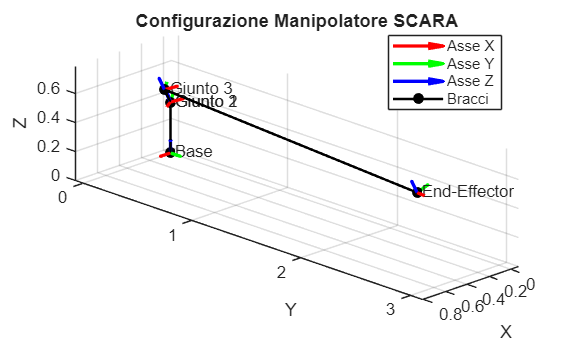
\includegraphics[width=1\linewidth]{figure_0.png}
\end{center}

\end{document}
